\section{Clouds}

For many observed spectra in the retrieval of exoplanet and brown dwarf atmospheres, a cloud model is required.  
In practical analyses, cloud models are often treated as a gray, spectrally flat, continuous opacity.  
Here, however, we introduce models that delve into cloud microphysics\footnote{For an in-depth discussion of cloud microphysics, see Pruppacher and Klett \cite{pruppacher2010microstructure}.}.  
In particular, we present the cloud model of Ackerman and Marley \cite{ackerman2001precipitating}, a seminal paper on exoplanet cloud modeling.  
Clouds form when atmospheric gas is assumed to condense into solids or liquids.  
In Earth’s atmosphere, clouds are primarily due to H$_2$O and occur as liquid-water clouds and ice clouds.  
Table~\ref{tab:input2} lists the main condensate species considered for exoplanets and brown dwarfs.

\begin{table}[!tbh]
\begin{center}
\caption{Typical cloud particle constituents and their material densities.\label{tab:input2}}
\begin{tabular}{lcc}
  \hline\hline
  Common name & Formula & Material density \\
  & & $\delta_\cond \ (\mathrm{g/cm^{3}})$ \\
  \hline
water & H$_2$O & 1 \\
& NH$_3$ & \\
Fe (solid) & Fe & 7.875 \\
ferrous oxide & FeO & 5.987 \\
phosphate & H$_3$PO$_4$ & \\
& KCl & \\
& Na$_2$S & \\
& TiO & \\
& SiC & \\
& VO & \\
hematite     & Fe$_2$O$_3$ & 5.275 \\
magnetite    & Fe$_3$O$_4$ & 5.200 \\
fayalite     & FeSiO$_4$ & 4.393 \\
corundum     & Al$_2$O$_3$ & 3.987 \\
quartz       & SiO$_2$ & 2.648 \\
rutile       & TiO$_2$ & 4.245 \\
enstatite    & MgSiO$_3$ & 3.194 \\
forstelite   & Mg$_2$SiO$_4$ & 3.214 \\
\end{tabular}
\end{center}
\end{table}

\subsection*{Terminal Velocity of Cloud Particles}\label{ss:termv}

Consider a cloud particle falling until it reaches a steady speed at which the drag force $F_d$ plus buoyant force $F_a$ balances gravity.  
This speed is called the terminal velocity. The force balance is
\begin{align}
F_d + F_a = m (r) g,
\end{align}
where $m(r)$ is the particle mass and $g$ is gravitational acceleration.  
Let $\delta_\cond$ be the material density of the condensate and $\rho$ the atmospheric density. Then
\begin{align}
m(r) &= \frac{4 \pi}{3} r^3 \delta_\cond, \\
F_a &= \frac{4 \pi}{3} r^3 \rho g,
\end{align}
so that
\begin{align}
\label{eq:Fd}
F_d &= \frac{4 \pi}{3} r^3 (\delta_\cond - \rho) g \\
&\approx  \frac{4 \pi}{3} r^3 \delta_\cond g,
\end{align}
where the last approximation neglects buoyancy since typically $\delta_\cond \gg \rho$.

In general, the drag force $F_d$ can be written in terms of the terminal velocity $v_f$ and the drag coefficient $C_d$ as
\begin{align}
F_d = C_d \frac{\rho v_f^2}{2} (\pi r^2),
\end{align}
(derivation omitted).  
Using the dimensionless Reynolds number
\begin{align}
\label{eq:Reynolds}
N_{re} = \frac{2 \rho v_f r}{\eta},
\end{align}
we can rewrite
\begin{align}
F_d = 6 \pi \eta r v_f \left( \frac{C_d N_{re}}{24} \right),
\end{align}
and combining with Eq.~(\ref{eq:Fd}) gives
\begin{align}
\label{eq:gcloud}
v_f(r) = \frac{2}{9 \eta}  g r^2 (\delta_\cond - \rho) \left( \frac{C_d N_{re}}{24} \right)^{-1},
\end{align}
where $\eta$ is the dynamic viscosity.

The coefficient $C_d$ depends on the Reynolds number.  
For $N_{re} \ll 1$ (Stokes flow),
\begin{align}
C_d = \frac{24}{N_{re}}.
\end{align}
For very small particles, slip at the particle surface becomes important; the Cunningham slip correction $(1+1.26 N_{Kn})$, with $N_{Kn}=k_B T/\sqrt{2 \pi r^2 P L}$ the Knudsen number, is applied.  
The resulting terminal velocity is
\begin{align}
\label{eq:sfcloud}
v_f^{sf}(r) = \frac{2}{9 \eta} g r^2 (\delta_\cond - \rho) (1+1.26 N_{Kn}),
\end{align}
which scales as $r^2$.  
At larger Reynolds numbers such a simple approximation is not valid; however, for $N_{re} \approx 0.01$--$300$, $v_f$ is roughly proportional to $r$, and for $N_{re} > 300$ it is roughly proportional to $r^{1/2}$.

For the dynamic viscosity, Rosner \cite{rosner2012transport} gives
\begin{align}
\label{eq:dyvis}
\eta = \frac{5}{16} \frac{\sqrt{\pi m k_B T}}{\pi d^2} \frac{(k_B T/\varepsilon)^{0.16}}{1.22},
\end{align}
where Rosner \cite{rosner2012transport} tabulates the molecular diameter $d$ and the Lennard–Jones potential parameter relative to $k_B$ for various atmospheric species.

At intermediate Reynolds numbers, consider the Davies number\footnote{Also called the Best number.} $N_D = C_d N_{re}^2$.  
Eliminating $v_f$ from Eq.~(\ref{eq:gcloud}) using the definition in Eq.~(\ref{eq:Reynolds}), we obtain
\begin{align}
\label{eq:davies}
N_D = C_d N_{re}^2 = \frac{32}{3 \eta^2} g r^3 \rho (\delta_\cond - \rho).
\end{align}

Using an empirical fit $y=f(x)$ to the measured relation between $x=\log{N_D}$ and $y=\log{N_{re}}$, we find $N_{re}$, and from Eq.~(\ref{eq:Reynolds}) the terminal velocity becomes
\begin{align}
\label{eq:vfmid}
v_f = \frac{\eta}{2 \rho r} e^{f(\log{N_D})}.
\end{align}

Using the values in Table 10.1 of Pruppacher and Klett \cite{pruppacher2010microstructure}, the fit
\begin{align}
\label{eq:daviesn}
f(x) = -0.0088 x^2 + 0.85 x - 2.49
\end{align}
works well (Fig.~\ref{fig:davies}).  
For $N_{re}>500$, following Ackerman and Marley (2001) \cite{ackerman2001precipitating}, we adopt $C_d=0.45$, yielding
\begin{align}
\label{eq:vflarge}
v_f = \frac{\eta}{2 \rho r} \sqrt{\frac{N_D}{C_d}}.
\end{align}

\begin{figure}[htb]
\begin{center}
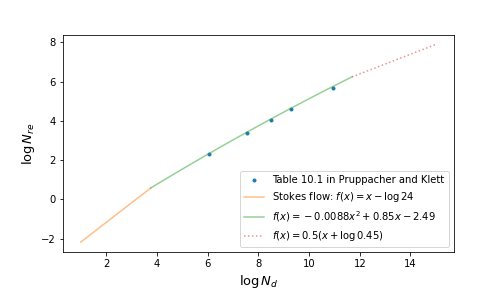
\includegraphics[width=\linewidth]{fig/clouds/davies_reynolds.png}
\caption{Relation between Davies number and Reynolds number.\label{fig:davies}}
\end{center}
\end{figure}

Summarizing, the terminal velocity is
\begin{align}
\label{eq:vterm}
v_f =
\begin{cases}
\displaystyle{\frac{2}{9 \eta} g r^2 (\delta_\cond - \rho) (1+1.26 N_{Kn}) } \\
\quad \mbox{for $N_D < 42$ ($N_{re} < 2$)}, \\[6pt]
\displaystyle{ \frac{\eta}{2 \rho r} \exp\!\big(-0.0088 \log^2{N_D}+0.85 \log{N_D} -2.49\big)} \\
\quad \mbox{for $42 \le N_D < 10^5$ ($2 \le N_{re} < 500$)}, \\[6pt]
\displaystyle{\frac{\eta}{2 \rho r} \sqrt{\frac{N_D}{C_d}}} \\
\quad \mbox{for $10^5 \ge N_D$ ($500 \ge N_{re}$)} 
\end{cases}
\end{align}
with boundary conditions chosen to ensure continuity.

\begin{figure}[htb]
\begin{center}
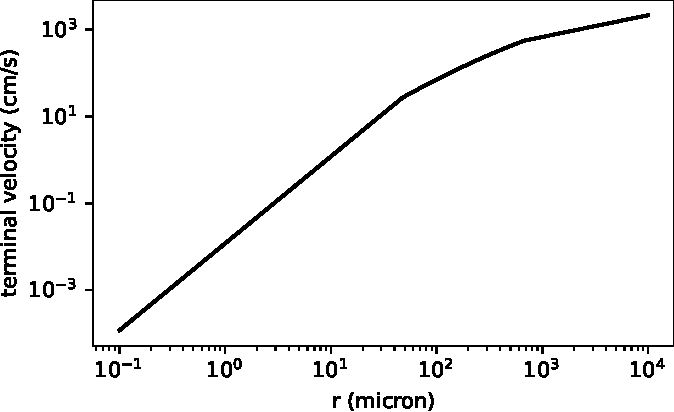
\includegraphics[width=\linewidth]{fig/clouds/vterm.pdf}
\caption{Cloud particle radius vs.\ terminal velocity for Earth’s atmosphere and gravity at $T=300$ K.\label{fig:vterm}}
\end{center}
\end{figure}

\begin{itembox}{Problem}
Consider water expelled by human conversation or breathing.  
According to the WHO definition, droplets with diameter $\geq 5\,\textmu m$ are called ``droplets,'' while those with diameter $\leq 5\,\textmu m$ are called ``aerosols'' or ``droplet nuclei.''  
If aerosols with diameter $5\,\textmu m$ are emitted from a mouth located $1.5$ m above the ground, how many minutes do they remain suspended in still air (neglecting airflow and evaporation)?
\end{itembox}

\subsection*{Vapor Pressure Curve and Cloud Base}

Consider clouds formed by phase transitions of a single constituent between gas–solid or gas–liquid.  
Clouds form when, above some altitude, the gas undergoes a phase transition into a solid or liquid.  
While cloud formation and dissipation involve complex physics, here we simply define the cloud base as the height at which the vapor pressure curve equals the partial pressure.  
Let the volume mixing ratio of the gaseous constituent be $\xi_v(P)$.  
Then the cloud base is the $(P,T)$ satisfying
\begin{align}
P(T) = P_\mathrm{sat}(T)/\xi_v(P),
\end{align}
as illustrated in Fig.~\ref{fig:pbase}.  
The saturation vapor pressure $P_\mathrm{sat}(T)$ can be written, using the latent heat $l$ and the Clausius–Clapeyron relation, as
\begin{align}
P_\mathrm{sat}(T) = P_\mathrm{sat,0} e^{-l/RT}
\end{align}
(Exoplanet Exploration, §6.2.3, p.~153).

For clouds composed of multiple gaseous constituents, there remains the question of how to determine the ``gaseous constituent'' volume mixing ratio $\xi_v(P)$.  
One may compute it via chemical equilibrium, or assume the maximum producible amount.  
In the latter approach, for example, for enstatite ($\mathrm{MgSiO_3}$), the limiting reagent determined from the elemental volume mixing ratios gives
\begin{align}
\xi_v = \mathrm{min}\,[ \,\xi(\mathrm{Mg}),\ \xi(\mathrm{Si}),\ \xi(\mathrm{O})/3 \, ].
\end{align}

%Ackerman and Marley cloud model.ipynb (exojax)
\begin{figure}[htb]
\begin{center}
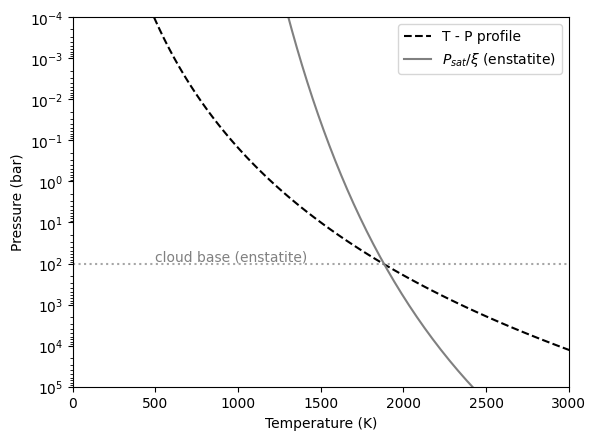
\includegraphics[width=\linewidth]{fig/clouds/pbase.pdf}
\caption{Definition of the cloud base. The intersection of the temperature–pressure profile with the vapor pressure curve divided by the volume mixing ratio gives the cloud base. \label{fig:pbase}}
\end{center}
\end{figure}

\subsection*{Ackerman and Marley Cloud Distribution Model}

We outline, with several modifications, the Ackerman \& Marley (2001) \cite{ackerman2001precipitating} (AM01) model, which is widely used for clouds in exoplanet and brown dwarf atmospheres.  
For simplicity, consider a single species that condenses to form clouds.  
For example, water clouds in an atmosphere have two states: the gaseous state ($\vapor$) and the condensed (cloud) state ($\cond$).  
We denote the sum of the two by $\total$.  
To avoid confusion, we consider mass mixing ratios rather than volume mixing ratios\footnote{For volume (number) mixing ratios, one must define what is being counted. For instance, one might count the total number of molecules in all cloud particles, or the sum of the numbers of cloud particles themselves, whose sizes—and thus molecular counts—differ.}.  
The total mass mixing ratio $X_\total (z)$ is the sum of the cloud mass mixing ratio $X_\cond(z)$ and the gas mass mixing ratio $X_\vapor (z)$:
\begin{align}
X_\total (z) = X_\cond (z) + X_\vapor (z).
\end{align}

The basic equation balances vertical transport against sedimentation (precipitation) of condensates, assuming a representative particle size:
\begin{align}
\label{eq:AM01}
- \Kzz \frac{\partial}{\partial z} X_\total (z) \;-\; \overline{v}_f (z)\, X_\cond (z) \;=\; 0,
\end{align}
where $\Kzz(z)$ is the vertical eddy diffusivity (units $\mathrm{cm^2/s}$), and $\overline{v}_f(z)$ is the typical settling velocity of cloud particles.

To solve Eq.~(\ref{eq:AM01}), we need an additional constraint among the three $X$’s.  
Here we assume
\begin{align}
\frac{X_\cond (z)}{X_\total (z)} = \mathrm{const.} \equiv k_c.
\end{align}
Then the differential equation becomes
\begin{align}
\label{eq:AM01c}
\frac{\partial}{\partial z} X_\cond (z) = - \frac{ k_c \,\overline{v}_f (z)}{\Kzz(z)} \, X_\cond (z).
\end{align}

From Eq.~(\ref{eq:AM01c}), if we may assume $\overline{v}_f (z) \propto \Kzz(z)$, the ODE is easily solved.  
AM01 effectively imposes such an assumption: the settling velocity $\overline{v}_f(z)$ is proportional to the vertical eddy velocity scale $v_\mathrm{eddy}(z)=\Kzz(z)/L$, where $L$ is a characteristic convective length scale taken as a constant\footnote{AM01 also presents a formulation where this is not constant; the constant case is presented as a heuristic.}.  
With a constant $\fsed$, we assume
\begin{align}
\overline{v}_f(z) = \fsed\, v_\mathrm{eddy}(z) = \fsed\, \Kzz(z)/L \\
\qquad\text{(the $\fsed$ assumption)} \nonumber
\end{align}
In this case, above the cloud base the solution is
\begin{align}
\label{eq:AM01cx}
X_\cond (z) = X_\cond(0) \exp\!\left( - \frac{ k_c \fsed}{L} \, z \right).
\end{align}

Assuming $L=H(z{=}0)=H_0$ and that the $z$–$P$ relation is determined hydrostatically by $H_0$, Eq.~(\ref{eq:AM01cx}) can be written
\begin{align}
X_\cond(P) = 
\begin{cases}
X_\cond(0) \left( \dfrac{P}{P_0} \right)^{\! f_{sed}/k_c}, & P \le P_0, \\[4pt]
0, & P > P_0,
\end{cases}
\end{align}
where $P=P_0$ is the cloud-base pressure.  
An example cloud mixing-ratio profile is shown in Fig.~\ref{fig:vmrcloud}.

%Ackerman and Marley cloud model.ipynb (exojax)
\begin{figure}[htb]
\begin{center}
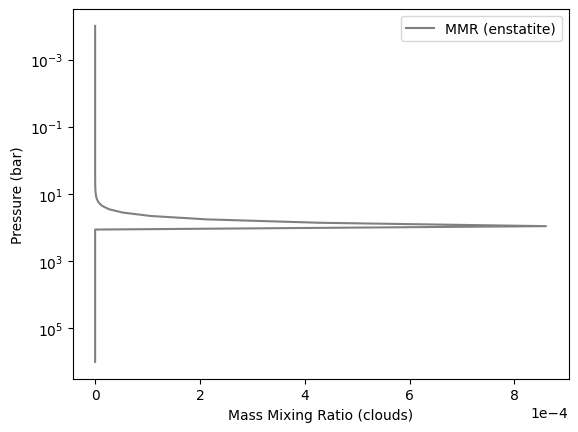
\includegraphics[width=\linewidth]{fig/clouds/mmrcloud.png}
\caption{Example of a cloud mass mixing ratio profile.\label{fig:vmrcloud}}
\end{center}
\end{figure}

We now introduce a particle size distribution.  
Define the number density of cloud particles per unit radius as
\begin{align}
    q(r) \equiv \frac{d \mathcal{N}_\cond (r)}{d r},
\end{align}
where $\mathcal{N}_\cond(r)$ is the number density of particles with radii $\le r$.  
Thus,
\begin{align}
    \int_0^\infty q(r)\, dr \;=\; \int_0^\infty \frac{d \mathcal{N}_\cond (r)}{d r} \, dr \;=\; \mathcal{N}_\cond (\infty) \equiv N,
\end{align}
the total number density of cloud particles.  
We use the symbol $N$ (instead of the gas number density symbol $n$) to emphasize that we are not counting the number of molecules but the number of particles.  
If $n_\cond$ denotes the number density of molecules constituting the cloud particles, then the mass mixing ratio relates as
\begin{align}
    X_\cond = \frac{\rho_\cond}{\rho} = \frac{\mu_\cond}{\mu} \frac{n_\cond}{n},
\end{align}
where ${\mu_\cond}$ is the molecular weight of the condensate species.  
Here $\rho_\cond$ is the mass density occupied by all cloud particles per unit volume of atmosphere ($\mathrm{g/cm^3}$).  
Do not confuse this with the intrinsic material density of a particle $\delta_\cond$ (also in $\mathrm{g/cm^3}$).

Let $m_\cond$ be the mass of an individual cloud particle; then $dm_\cond/dr$ is the mass distribution with respect to radius.  
Assuming spherical particles,
\begin{align}
    \frac{dm_\cond}{dr} = \frac{4}{3} \pi r^3 \delta_\cond \frac{d \mathcal{N}_\cond (r)}{d r} = \frac{4}{3} \pi r^3 \delta_\cond\, q(r).
\end{align}

While $\Kzz$ and the settling speed $v_f(z;r)$ at each particle size $r$ could be specified individually, the $\fsed$ assumption generally does not hold if treated strictly size-by-size.

A strongest (but restrictive) way to enforce the $\fsed$ assumption is to set, for each size,
\begin{align}
v_f(z; r)= \fsed\, v_\mathrm{eddy}(z) = \fsed\, \Kzz(z)/L,
\end{align}
but this loses the size dependence of the settling velocity.  
Indeed, Eq.~(\ref{eq:AM01}) is not asserted to hold for every particle size but for some representative value; hence we push the $\fsed$ assumption onto the representative averaging.

Let the representative operation for settling speed be the mass-weighted mean:
\begin{align}
\label{eq:fsedw}
&\overline{v}_f(z) 
= \frac{\int v_f(m_\cond)\, dm_\cond}{M_c(z)}
= \frac{\int_0^\infty v_f(z; r)\, (dm_\cond/dr)\, dr}{ \int_0^\infty (dm_\cond/dr)\, dr } \nonumber \\
&= \frac{\int_0^\infty dr \, v_f(z;r)\, r^3 q(r)}{ \int_0^\infty dr \, r^3 q(r)},
\end{align}
where the total cloud mass per unit volume at height $z$ is $M_c(z)=X_\cond(z)\,\rho$ (with $\rho$ the atmospheric mass density).

To satisfy the $\fsed$ assumption, we require
\begin{align}
\label{eq:fsedw2}
\fsed\, \frac{\Kzz(z)}{L} 
= \frac{\int_0^\infty dr \, v_f(z;r)\, r^3 q(r)}{ \int_0^\infty dr \, r^3 q(r)}.
\end{align}

AM01 assumes a lognormal size distribution in the layer at height $z$:
\begin{align}
\label{eq:lognormal_am01}
&q(r)\, dr = N(z)\, p_z(r)\, dr \qquad\text{(lognormal size distribution)}, \\
&p_z(r) = \nonumber \\
&\frac{1}{r \sqrt{2 \pi}\, \log{\sigma_g}} 
\exp\!\left\{ - \frac{1}{2 (\log{\sigma_g})^2} \left[\log\!\left(\frac{r}{r_g(z)}\right)\right]^{\!2} \right\},
\end{align}
with $\log{\sigma_g}>0$ ($\sigma_g>1$)\footnote{In the usual notation for the lognormal distribution, $\sigma$ would denote what we write as $\log{\sigma_g}$; here we follow AM01, acknowledging the potential for confusion.}.  
Note that $\sigma_g$ controls the distribution width, and AM01 adopts a common value across layers.  
Using the moment formula for the lognormal distribution,
\begin{align}
E_k \equiv \int_0^\infty r^k\, p_z(r)\, dr \;=\; r_g^k(z)\, \exp\!\left(\frac{k^2 \log^2{\sigma_g}}{2}\right),
\end{align}
we have
\begin{align}
&M_c(z) = X_\cond \rho 
= \int dr \, \frac{4 \pi \delta_\cond r^3}{3}\, q(r) \nonumber \\
&= N(z) \frac{4 \pi \delta_\cond r_g^3(z)}{3} \exp\!\left(\frac{9}{2}\log^2 \sigma_g\right),
\end{align}
so the particle number density $N(z)$ is
\begin{align}
\label{eq:lognormal_am01N}
N(z) &= \frac{X_c \rho}{\tilde{m}}, \\ 
\label{eq:lognormal_mean_mass}
\tilde{m} &\equiv \frac{4 \pi r_g^3}{3}\, \delta_c \, \exp\!\left(\frac{9}{2} \log^2{\sigma_g} \right),
\end{align}
where $\tilde{m}$ is interpreted as the mean mass per particle linking cloud mass density to number density.

From the requirement in Eq.~(\ref{eq:fsedw2}),
\begin{align}
\label{eq:xaxax}
 \int_0^\infty dr \, v_f(z;r)\, r^3 q(r) \;=\; \fsed\, \frac{\Kzz(z)}{L}\, E_3,
\end{align}
we must assume a form for $v_f(r; z)$.  
From the previous section, despite some dependence on Reynolds number, the terminal velocity approximately follows a power law in $r$.  
Thus we assume a power-law settling speed
\begin{align}
v_f(r,z) = A\, r^\alpha \qquad\text{(power-law settling assumption)}.
\end{align}

From Eq.~(\ref{eq:xaxax}), we obtain
\begin{align}
\label{eq:xaxax2}
 A &= \frac{\Kzz(z)}{r_g^\alpha(z)} \frac{\fsed}{L} \frac{E_3}{E_{\alpha+3}} \nonumber \\
 &= \frac{\Kzz(z)}{r_g^\alpha(z)} \frac{\fsed}{L}\, 
 \exp\!\left[ -\frac{\alpha^2 + 6 \alpha}{2}\, \log^2{\sigma_g} \right],
\end{align}
so that
\begin{align}
\label{eq:xaxax2x}
 v_f(r;z) &= \frac{\Kzz(z)}{r_g^\alpha(z)} \frac{\fsed}{L}\,
 \exp\!\left[ -\frac{\alpha^2 + 6 \alpha}{2}\, \log^2{\sigma_g} \right] r^\alpha \\
  &= \frac{\Kzz(z)}{L} \left( \frac{r}{r_w(z)} \right)^\alpha,
\end{align}
where
\begin{align}
\label{eq:lognormal_am01rg}
r_w(z) = r_g(z)\, \fsed^{-1/\alpha}\, \exp\!\left[ \left(\frac{\alpha+6}{2} \right) \log^2{\sigma_g}\right].
\end{align}
With this distribution, the $\fsed$ assumption holds.  
Because Eq.~(\ref{eq:xaxax2x}) is a power law, $r_w(z)$ does not set a typical scale per se; it merely gives, at a given $z$, the particle size whose settling velocity balances vertical mixing.

To close the system we must determine $r_g(z)$ and $\alpha$.  
For $r_g(z)$, one may use the physical terminal-velocity model of §\ref{ss:termv} to find the $r$ such that $v_f(r)=\Kzz(z)/L$, then identify that with $r_w$ and infer $r_g$ via Eq.~(\ref{eq:vterm}).  
AM01 further recommends fitting $\alpha$ by matching the $r$-dependence of the physically motivated terminal-velocity model near this range.

\begin{itembox}{Features of the AM01 Cloud Model (constant $k_c$ and $\fsed$)}
Given $\fsed$, $\Kzz(z)$, $\sigma_g$, and $k_c$, the vertical distribution of the cloud mixing ratio in each layer is given by Eq.~(\ref{eq:AM01cx}), and—assuming a lognormal size distribution—the particle size distribution in each layer is specified by Eqs.~(\ref{eq:lognormal_am01}), (\ref{eq:lognormal_am01N}), and (\ref{eq:lognormal_am01rg}).
\end{itembox}

With the abundance of each particle size known for each layer, the cloud cross section follows by summing the scattering cross sections (Rayleigh or Mie) over the size distribution.

\subsection*{Cross Section When Size Dependence Is Negligible}

Consider the extinction cross section when the extinction efficiency $Q_e(r)$ is constant, independent of particle size:
\begin{equation}
    Q_e (r) = Q_e \qquad \text{(constant)}.
\end{equation}
The same development applies for absorption and scattering by replacing $Q_e$ with $Q_a$ or $Q_s$.

\begin{align}
\overline{\sigma}_\mathrm{ext}(z) &= \frac{\int_0^\infty dr \, Q_e \pi r^2 q(r)}{N} \\
&=  Q_e \pi r_g^2(z)\, e^{2\log^2{\sigma_g}} \;\equiv\; Q_e \pi \overline{r}_\mathrm{geo}^2,
\end{align}
defining the mean geometric radius
\begin{align}
\overline{r}_\mathrm{geo} \equiv e^{\log^2{\sigma_g}}\, r_g 
= r_w(z)\, \fsed^{1/\alpha}\, \exp\!\left[-\frac{\alpha+4}{2}\, \log^2{\sigma_g}\right].
\end{align}

The optical depth increment in each atmospheric layer is then
\begin{align}
d \tau &= \int_0^\infty dr \, Q_e \pi r^2 q(r)\, dz \;=\; N\, \overline{\sigma}_\mathrm{ext}(z)\, dz \\
&= Q_e \pi \overline{r}_\mathrm{geo}^2\, N\, dz.
\end{align}
This expresses the optical depth in terms of the mean geometric radius and the particle number density.  
Using Eqs.~(\ref{eq:lognormal_am01N}) and (\ref{eq:lognormal_mean_mass}), we can convert from number density to mass-density form:
\begin{align}
\label{eq:dtaucloud0}
d \tau &= \frac{3  \rho Q_e }{4 \delta_\cond r_g(z)} 
\exp\!\left[ - \frac{5}{2} \log^2{\sigma_g} \right]  X_\cond (P)\, dz \\
&= X_\cond  (z)\, \frac{3 \rho Q_e }{4 \delta_\cond r_w(z)\, \fsed^{1/\alpha}}  
\exp\!\left[ \left( \frac{\alpha + 1}{2} \right) \log^2{\sigma_g} \right] dz \\
\label{eq:dtaucloud1}
&= \frac{3 Q_e\, X_\cond  (z)\, \rho}{4 \delta_\cond\, r_\mathrm{eff}(z)} \, dz,
\end{align}
where, following AM01, we defined the effective radius
\begin{align}
r_\mathrm{eff}(z) &\equiv r_w(z)\, \fsed^{1/\alpha}\, \exp\!\left[ - \left( \frac{\alpha + 1}{2} \right) \log^2{\sigma_g} \right] \\
&= r_g(z)\, \exp\!\left[ \frac{5}{2} \log^2{\sigma_g} \right].
\end{align}
Note that this definition does not coincide with the mean geometric radius.

Using Eq.~(\ref{eq:dtaucloud0}) and converting to pressure coordinates via Eq.~(\ref{eq:pressureeq_}), we obtain
\begin{align}
d \tau &=  \frac{3 Q_e\, X_\cond (z)}{4 r_g\, \delta_\cond\, g}  
\exp\!\left(- \frac{5}{2} \log^2{\sigma_g}\right) dP,
\end{align}
which emphasizes that $(r_g,\sigma_g)$ are the inputs.

Overall,
\begin{align}
\tau &= - \int_0^{P_0} X_\cond (P)\, \frac{3  Q_e\, \rho}{4 \delta_\cond\, r_\mathrm{eff}} 
\left( \frac{dz}{dP} \right) dP \\
&=  X_\cond (0) \int_0^{P_0}  dP \; \frac{3 Q_e\, \rho}{4 \delta_\cond\, r_\mathrm{eff}}  \frac{H}{P} 
\left( \frac{P(z)}{P_0} \right)^{f_{sed}/k_c}\\
&\approx   \frac{3}{4} \frac{ Q_e\, X_\cond(0)\, P_0}{ \delta_\cond\, g\, r_\mathrm{eff}\, (1 + \fsed k_c) },
\end{align}
where the last step used $P_0/H = g \rho_0$ and $\rho \approx \rho_0$ (Exoplanet Exploration, p.~137, Eqs.~6.5 and 6.6, and p.~139, Eq.~6.28)\footnote{The corresponding AM01 Eq.~(18) contains a typographical error missing a factor of $1/\delta_\cond$.}.  
In general $Q_e$ depends on size, but in the large-particle limit $Q_e \to 2$, yielding the geometric cross section.

\subsection*{Cross Section for Mie Scattering}

In general, using the size-dependent extinction efficiency $Q_e(r)$ from Mie theory,
\begin{align}
d \tau &= \int_0^\infty dr \, Q_e (r)\, \pi r^2\, q(r)\, dz,
\end{align}
one computes the optical depth.  
Although Mie calculations can be demanding, convenient software exists; for example, {\sf PyMieScatt} is a Python-based Mie-scattering package.
